\documentclass[english]{article}
\usepackage[T1]{fontenc}
%\usepackage[latin9]{inputenc}
%\usepackage{geometry}
%\geometry{verbose,tmargin=1in,bmargin=1in,lmargin=1in,rmargin=1in}
\usepackage{amsmath}
\usepackage{amssymb}
\usepackage{setspace}
\usepackage[utf8]{inputenc}
\usepackage{graphicx}
\usepackage{float}
\usepackage{adjustbox}
\usepackage{gensymb}
\usepackage{amssymb}
\usepackage{array}
\usepackage{ragged2e}
\usepackage{lipsum}
\onehalfspacing
\usepackage{babel}
\usepackage{ctable}
\usepackage{booktabs}
\usepackage{graphicx}
\usepackage{caption}
\usepackage{subcaption}

\begin{document}
\title{Informality Trend in LAC: Small and Disappointing Progress }
\maketitle
\begin{abstract}
    This descriptive paper uses household and employment surveys from the region to paint a more complete picture of the different aspects of informality. We show that there has been progress on increasing the share of dependent workers who contribute to social security but that the productive structure of the economies have remained unchanged. We argue that this is mainly coming from the focus of governments policies on facilitating the registration of low productivity workers, therefore subsidizing low productivity firms. To make this point we use two approaches: a qualitative approach based on the analysis of policies that have been identified as successful in reducing informality. Second, we use a simple decomposition on different formalization margins to show that the formalization process in the region has been dominated by workers transitioning to formal status in the same type of firm. This means that the progress made in formalizing workers has happened mainly through increasing coverage of workers in small firms. 
\end{abstract}
\section{Introduction}
\begin{itemize}
    \item Motivation: Informality is a pervasive problem in the region despite many attempts to curtail it. 
    \item The mainstream measure of informality comes from the ILO and includes many dissimilar phenomena. 
    \begin{itemize}
        \item Low productivity and unprotected workers
    \item There is a common understanding on the fact that informality is bad
    \item 
    \end{itemize}
\end{itemize}

\subsection{Regional figures}

\begin{figure}
\centering
  \caption{Evolution of alternative informality related measures}
\begin{subfigure}{.5\textwidth}
  \centering
  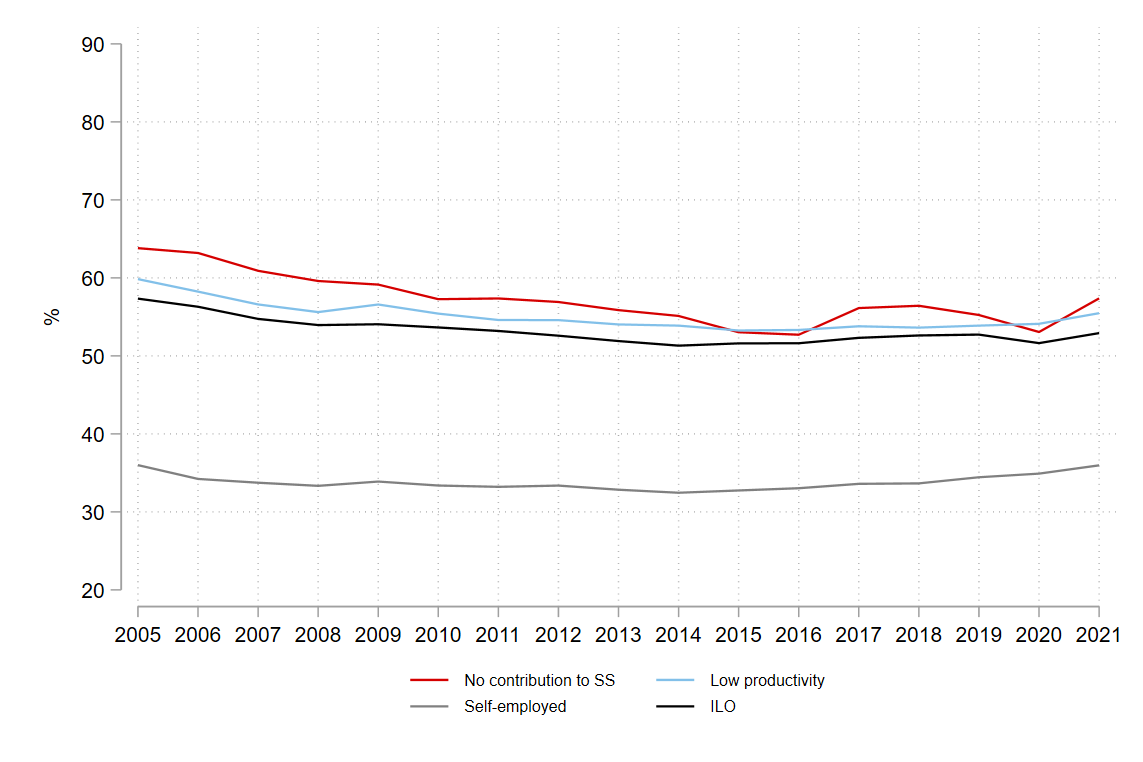
\includegraphics[width=1\linewidth]{latex/figures/LAC_ipo_fig1.png}
  \label{fig:sub1}
\end{subfigure}%
\begin{subfigure}{.5\textwidth}
  \centering
  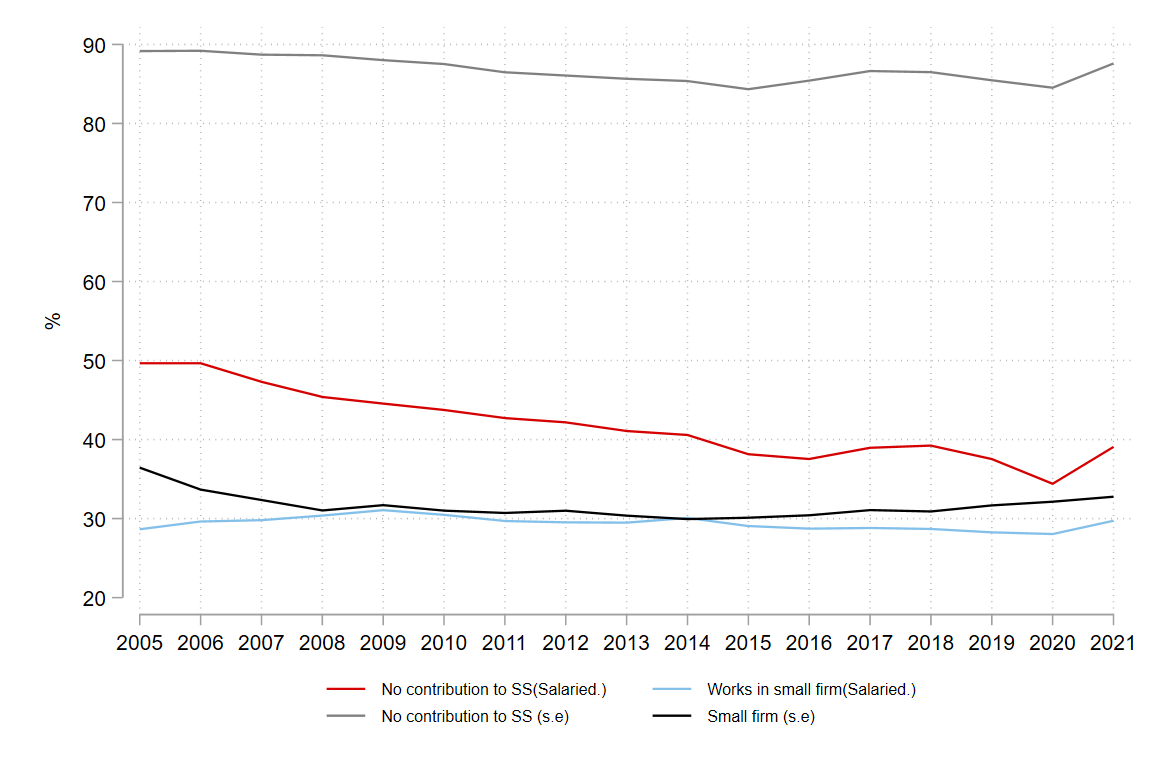
\includegraphics[width=1\linewidth]{latex/figures/LAC_ipo_fig2.png}
  \label{fig:sub2}
\end{subfigure}
\label{fig:test}
\source{Source: SEDLAC and ILO.}

\footnotesize{\note{Note SEDLAC: Both figures show unweighted means of country level indicators. The countries included in the sample are Argentina, Bolivia, Brazil, Colombia, Costa Rica, Ecuador, Honduras, Mexico, Panama, Peru, Paraguay, El Salvador and Uruguay. Some countries don’t have information for the entire period: Bolivia and Brazil have missing values in 2010; Colombia have missing values in 2006 and 2007; Honduras have missing values in 2020-2021; Mexico have missing values 2005, 2007, 2009, 2011, 2013, 2015, 2017, 2019, 2020, 2021; Panama and El Salvador have missing values 2020; and Uruguay have missing values in 2021. In that cases we interpolate the sample using the closest last year value. Note ILO: The serie is a modeled estimated informal employment rate by ILO. }}
\end{figure}

\subsection{Household cross country figures}

\subsection{Individual cross country figures}




\end{document}